\scanpage{89}
\mspage{85}
% archive sheet number: 88

et elle se prolonge aussitôt en une application
\[
\unsure{\alpha_*|\varphi_*|\alpha_{\times}}\text{ ou }\bar\alpha:
\unsure{\mathscr{P}|\mathcal{P}|\mathfrak{P}}(E)\unsure{{-}|\longrightarrow}\mathscr{P}(E')
\qquad\unsure{A|\mathbb{A}|\mathscr{A}}\mathbin{-}\bigcup_{x\in A}\alpha(x)
\]
% slanted
\margin{J'écris $\bar\alpha$ en pensant à des \unsure{parties} des ensembles $E,E'$ et $\alpha_*$ en pensant à une application entre \unsure{spotos|spatos}.}

Cette application $\bar\alpha$ commute aux $\operatorname{Sup}$ quelconques\inserted{(donc est croissante)}, et inversement, toute application $\varphi:\mathscr{P}(E)\mathbin{-}\mathscr{P}(E')$ qui a cette propriété, s'écrit de façon unique sous la forme $\alpha_*$, puisque $\deleted{\unsure{\forall}}A\in\mathscr{P}(E)$, on a
\[
A=\operatorname{Sup}_{x\in A}\{x\}\quad\text{donc}\quad
\varphi(A)=\operatorname{Sup}_{x\in A}\underset{\alpha(x)\,{}^{\text{``\unsure{def|déf}}}}{\underset{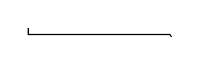
\begin{tikzpicture}[baseline=0pt]\draw (0,0.08)--(0,0)--(1.8,0)--(1.82,-0.03);\end{tikzpicture}}{\varphi(\{x\})}}
\]
% slanted
\margin{\unsure{Compatibilité} avec la \unsure{composition} des \unsure{correspondances}\figure{
\begin{tikzpicture}[x=1mm,y=1mm]\draw (0,26) .. controls (-1,20) and (-1,13) .. (1,12) -- (6,13) .. controls (1,9) and (1,6) .. (2,0);\end{tikzpicture}}}

Nous allons interpréter l'a\deleted{\unsure{pp|p}} correspondance symétrique, ou transposée, $\unsure{\beta|B}$ de $\alpha$, en termes de
\[
\beta_*\text{ ou }\bar\beta:\mathscr{P}(E')\longrightarrow\mathscr{P}(E),
\]
en \deleted{\unsure{tant}} termes des spotos $\mathscr{P}(E)$, $\mathscr{P}(E')$, en notant que
% Left-hand label as on the scan.
\begingroup
\makeatletter\tagsleft@true\makeatother
\[
\left\{\begin{aligned}
&\forall A\in\mathscr{P}(E),\ A'\in\mathscr{P}(E')\quad\text{on a}\\
&\alpha_*(A)\mathrel{|{\circ}|}A'\Longleftrightarrow A\mathrel{|{\circ}|}\beta_*(A')
\end{aligned}\right.
\tag*{\unsure{a)|b)}}
\]
\endgroup
En effet, le premier \unsure{mb|m.b.} s'écrit
\[
\begin{aligned}
&\deleted{\unsure{\forall x\in A,}}\forall x'\in A',\quad\text{on a }x'\notin\bar\alpha(A)\quad\text{i.e. }\unsure{\nexists|\exists}x\in A\\
&\text{avec }x'\in\unsure{\alpha|\bar\alpha}(x)\quad\text{i.e. }(x,x')\in R
\end{aligned}
\]
ou encore
\[
\forall\unsure{x'|x}\in A,\ x'\in A'\quad\text{on a }(x,x')\notin R\quad\text{i.e. }(x,x')\in\bar R
\]
